% !TeX spellcheck = en_US
%%%%%%%%%%%%%%%%%%%%%%%%%%%%%%%%%%%%%%%%%%%%%%%%%%%%%%%%%%%%%%%%%%%%%%%%%%%%%%%%%%
% TOC and BIB
%%%%%%%%%%%%%%%%%%%%%%%%%%%%%%%%%%%%%%%%%%%%%%%%%%%%%%%%%%%%%%%%%%%%%%%%%%%%%%%%%%
\only<article>{
	%
	\maketitle
	\thispagestyle{empty}
	\setcounter{page}{0}
	%
	\newpage
	\tableofcontents
}





%%%%%%%%%%%%%%%%%%%%%%%%%%%%%%%%%%%%%%%%%%%%%%%%%%%%%%%%%%%%%%%%%%%%%%%%%%%%%%%%%%
% ORGANIZATION
%%%%%%%%%%%%%%%%%%%%%%%%%%%%%%%%%%%%%%%%%%%%%%%%%%%%%%%%%%%%%%%%%%%%%%%%%%%%%%%%%%
%%\only<presentation>{
%%
%\begin{frame}
%\vspace{3cm}
%\begin{center}
%	\LARGE \bf \color{header} ORGANIZATION
%\end{center}
%\end{frame}
%%
%\begin{frame}
%\textbf{\large\color{header} Organization}~\\\vspace{0.5cm}
%Always start from here:
%\begin{center}
%	\hyperref{https://www.math.uni-trier.de/~vollmann/elomath/}{}{}{https://math.uni-trier.de/\hspace{-0.06cm}${\tiny \sim}$\hspace{-0.1cm} vollmann/elomath/}
%\end{center}
%%
%\vspace{0.5cm}
%You can log in using the following credentials:
%%
%\begin{center}
%	\color{magenta}
%	User: \texttt{elomath-user}~~~ Password: \texttt{elomath-student-pwd}
%\end{center}
%%
%\vspace{1.5cm}
%In particular you will find an \textit{information sheet}, which contains \textbf{all} organizational information for this course (if you miss something please contact me: \href{mailto:vollmann@uni-trier.de}{vollmann@uni-trier.de}).
%~\\~\\~\\
%Video recordings as well as homework submissions and corrections will be uploaded on the platform \exerciseUploadRep.
%%\begin{center}
%%%	\includegraphics[width=0.8\textwidth]{cover3.jpg}
%%\end{center}
%\end{frame}
%%
%%
%%%%%%
%\begin{frame}
%\textbf{\large\color{header} Lecture}~\\\vspace{0.5cm}
%\begin{itemize}
%\item Mode: \textbf{digital}, 2x 90min
%\item Date and room:
%\begin{center}
%\lecturedates~~ in~~~\\ \exerciserooms.~\\~\\
%\end{center}
%\vspace{1cm}\item \textbf{Before} each lecture I will upload a set of thinned out slides on
%\begin{center}
%\slides .
%\end{center}
%\vspace{1cm}\item \textbf{After} the lecture I will upload a second version of these slides which contains the notes that were added during
%the lecture. If necessary, a video \textbf{recording} of my screen and input-audio will be uploaded on \exerciseUploadRep.
%\end{itemize}
%\end{frame}
%%
%%%%%%
%\begin{frame}
%\textbf{\large\color{header} Exercise Class}~\\\vspace{0.5cm}
%\begin{center}
%\includegraphics[width=0.4\textwidth]{\PathToMedia/cover6.jpg}
%\end{center}
%\begin{itemize}
%\item Mode: \textbf{digital}, 1x 90min
%\item Date and room:
%\begin{center}
%\exercisedates ~~via\\	\exerciserooms.\\
%\textit{(Depending on your schedules I would like to choose just one of these dates.)}
%\end{center}
%~\\
%\item The build will be uploaded every \exercisedatesUploadday~to:
%\begin{center}
%\build .
%\end{center}
%\end{itemize}
%\end{frame}
%\begin{frame}
%~\\
%\textbf{\large\color{header} Mandatory Submissions}~\\
%\begin{itemize}
%	\item Solutions have to be submitted on a weekly basis
%	\item In order to get admitted for the exam, it is necessary to reach an overall score of 50\% in \textbf{each} part, theoretical exercises (T) and programming exercises (P) 
%\end{itemize}
%%
%~\\~\\
%\textbf{\color{header} Remarks on the theoretical exercises}~\\
%\begin{itemize}
%	\item Everybody is asked to hand in a separate sheet for (T).
%	\item \textbf{\color{red}Submission:}\\ Upload a clearly readable .pdf--file containing your solutions for (T) in the respective \textit{Homework} folder in \exerciseUploadRep.
%	~\\~\\ For instance, you can generate such a .pdf--file in one of the following ways:
%	\begin{itemize}
%		\item Scan your handwritten notes (Scanner or smartphone app),
%		\item \textbf{Using \LaTeX},
%		\item Using a tablet with Stylus (e.g., iPad with Apple Pencil),
%		\item Using a graphics tablet (e.g., Wacom).
%	\end{itemize}
%\end{itemize}
%%
%\end{frame}
%%
%\begin{frame}
%~\\
%\textbf{\color{header} Remarks on the programming exercises}~\\
%\begin{itemize} \normalsize
%	\item Please solve the exercises in an IPython Jupyter Notebook using Python 3 (download \hyperref{https://www.anaconda.com/distribution/}{}{}{Anaconda}).
%	\item You are allowed to hand in your submission in groups of three members
%	\item \textbf{\color{red}Submission:}\\
%	 Upload the .ipynb file (IPython Notebook) containing your solutions for (P) to the respective \textit{Homework} folder in \exerciseUploadRep.\\~\\
%	 $\rightarrow$ The source code will be evaluated concerning functioning, readability and annotation.
%\end{itemize}
%%
%~\\~\\
%\textbf{\color{header} Corrections}~\\
%You will find the corrected submissions in the respective \textit{Homework} folder in \exerciseUploadRep
%\end{frame}
%%
%%%%%%
%\begin{frame}
%\textbf{\large \color{header} Exam}~\\\vspace{0.5cm}
%\begin{center}
%\includegraphics[width=0.3\textwidth]{\PathToMedia/exam.jpg}
%\includegraphics[width=0.3\textwidth]{\PathToMedia/comic.jpg}
%\includegraphics[width=0.3\textwidth]{\PathToMedia/comic2.eps}
%\end{center}
%\begin{itemize}
%\item Written exam over 120min (date tba)
%\vspace{0.5cm}\item \textbf{Mastering all exercises	will enable you to pass the exam!}
%\vspace{0.3cm}\item The lecture notes and especially the exercises are the relevant material for the exam. Studying related literature is still recommended and will help to broaden your view.
%\end{itemize}
%\end{frame}
%%
%%%%%%
%\begin{frame}
%\textbf{\large\color{header} Digital Format}~\\\vspace{0.5cm}
%\begin{center}
%\includegraphics[width=0.3\textwidth]{\PathToMedia/homeschool3.jpg}
%\includegraphics[width=0.3\textwidth]{\PathToMedia/homeschool2.jpg}
%\end{center}
%%\begin{itemize}
%%\item Lecture in presence as for now
%%\item Exercise class via Zoom
%%\end{itemize}
%~\\
%Minimal prerequisites:
%\begin{itemize}
%	\item Internet connection (if possible, I recommend to connect to your router with a LAN cable (Ethernet))
%	\item Web browser and loudspeakers (optional: microphone and camera)
%	\item Best: Use licensed Zoom account with university account and desktop client/App.
%\end{itemize}
%~\\
%I would very much appreciate to see your faces: \textbf{Please turn on your video!}
%~\\~\\
%
%% 
%\end{frame}
%%
%%%%%%
%\begin{frame}
%\textbf{\large \color{header} Questions and Feeback}~\\\vspace{0.5cm}
%
%\begin{itemize}
%\item Do not hesitate to contact me -- at best \textbf{during the classes} (questions often relate to others, too)\\
%\begin{itemize} \normalsize
%\item Simply turn on your microphone and interrupt me (I may oversee the chat sometimes)! 
%\item I will be the last one who leaves the zoom room so that you may have the opportunity to ask questions with a reduced audience in the end.
%\end{itemize} 
%\vspace{1cm}\item I am always happy to get suggestions for improvement throughout the course! 
%\end{itemize} 
%\end{frame}
%


%%%%%%%%%%%%%%%%%%%%%%%%%%%%%%%%%%%%%%%%%%%%%%%%%%%%%%%%%%%%%%%%%%%%%%%%%%%%%%%%%%%
%% APPETIZER
%%%%%%%%%%%%%%%%%%%%%%%%%%%%%%%%%%%%%%%%%%%%%%%%%%%%%%%%%%%%%%%%%%%%%%%%%%%%%%%%%%%
%%
%\begin{frame}
%\vspace{5cm}
%\begin{center}
%	\LARGE \bf \color{header} CONTENT 
%\end{center}
%\end{frame}

%
\begin{frame}
	\Section{A Short Introduction to the Topic}
	~\\
	\elomath{\text{From the Module Handbook:}\\~\\
		\textit{``After completing the module, the students know the mathematical foundations in the areas of linear algebra and \textbf{numerical mathematics}. As part of the course, they acquire or deepen knowledge in the programming language \textbf{Python}.''}}
	~\\
	\textbf{Numerical mathematics?}\\~\\
	\textit{From Wikipedia: Field of mathematics that deals with the construction and analysis of algorithms to approximately (but accurately) compute solutions to (hard) continuous problems -- typically using computers.}
	~\\~\\~\\~\\
	\textbf{Why is this important?}~\\
	\begin{itemize}
		\item most (all?) \textbf{application}-oriented problems cannot be solved exactly $\rightarrow$ \textit{\textbf{hard}} problems \vspace{0.3cm}
	\end{itemize}
	\begin{minipage}[t]{0.25\textwidth}\centering
		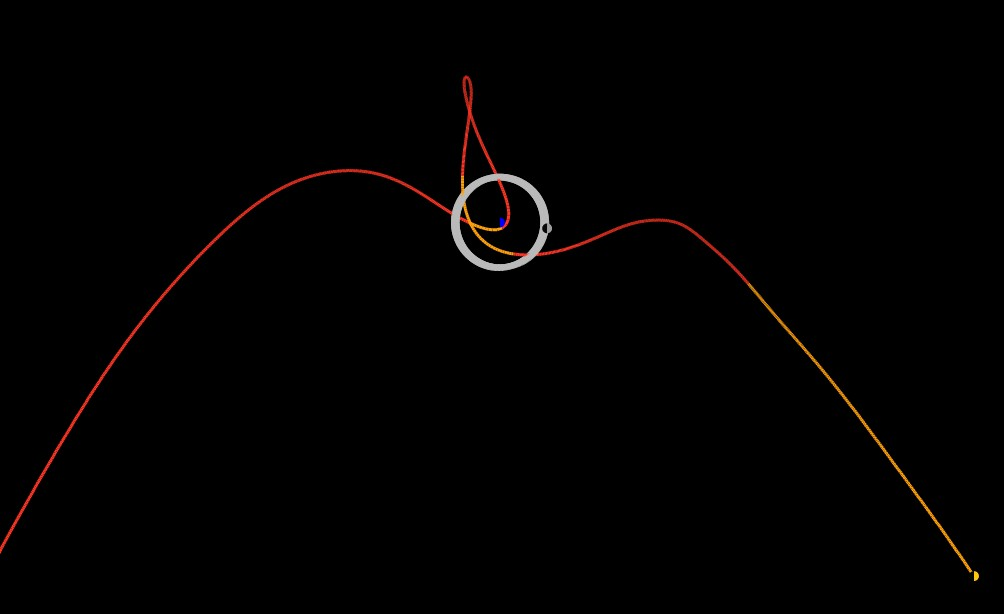
\includegraphics[width=\textwidth]{\PathToMedia/trajectories_2020SO.jpg}\\
		trajectories of objects in space \\
		\hyperref{https://en.wikipedia.org/wiki/2020_SO\#/media/File:2020SO_b.gif}{}{}{2020SO} 
	\end{minipage}
	\begin{minipage}[t]{0.25\textwidth}\centering
		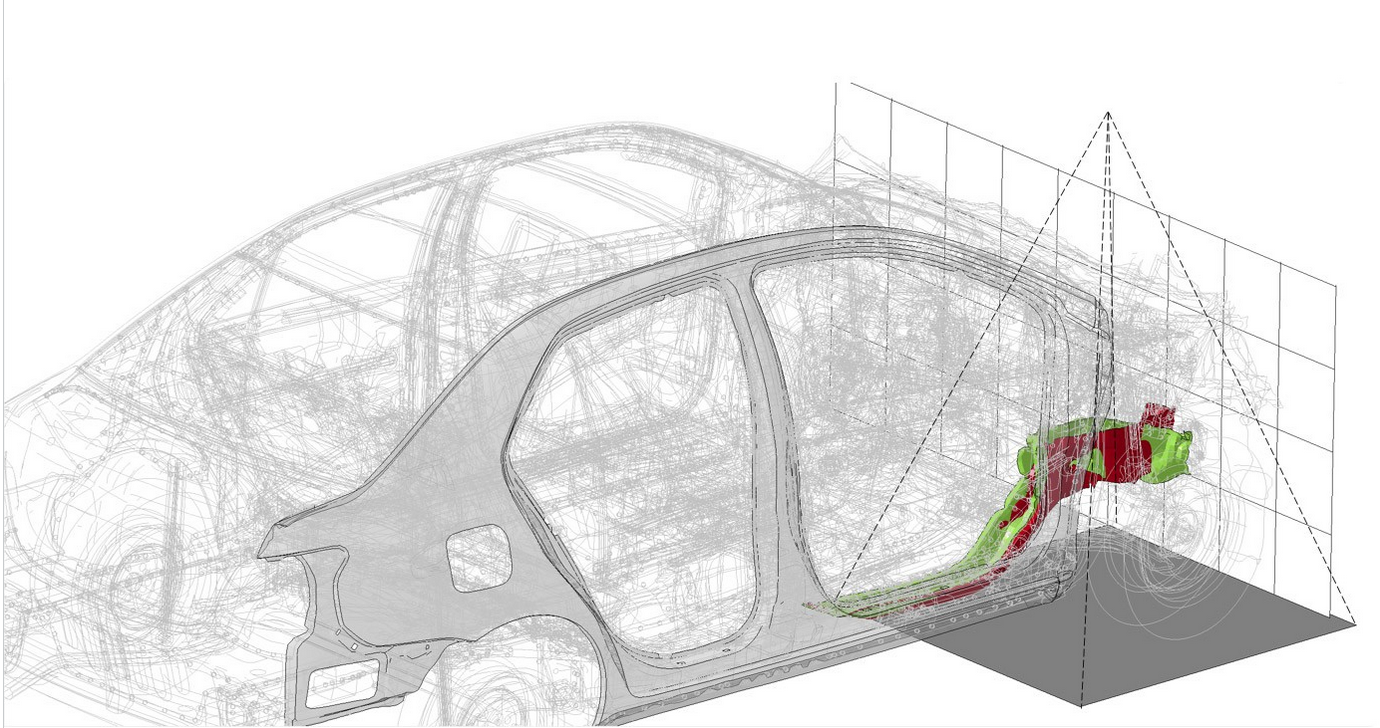
\includegraphics[width=\textwidth]{\PathToMedia/carcrash_sim.png}\\
		\hyperref{https://www.emi.fraunhofer.de/de/geschaeftsfelder/automotive/forschung/archiv/Roentgen-Crashtest.html}{}{}{car crash simulation} 
	\end{minipage}
	\begin{minipage}[t]{0.25\textwidth}\centering
		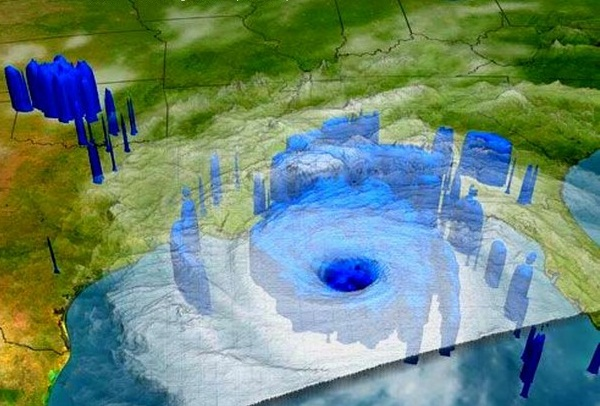
\includegraphics[width=\textwidth]{\PathToMedia/weather.jpg}\\
		\hyperref{https://en.wikipedia.org/wiki/Numerical_weather_prediction}{}{}{weather prediction} 
	\end{minipage}
	% CT SCAN
	\begin{minipage}[t]{0.25\textwidth} \centering
		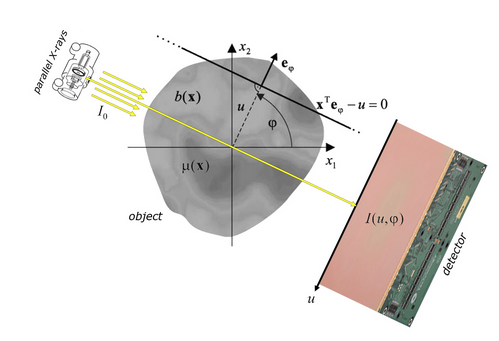
\includegraphics[width=\textwidth]{\PathToMedia/ct_scan.png}\\
		\hyperref{https://en.wikipedia.org/wiki/CT_scan}{}{}{CT Scan} 
	\end{minipage}
\end{frame}
%
\begin{frame}
	\textbf{\color{header} Relation to Data Science?}~\\
	\begin{itemize}
		\item \textbf{data}-driven models are more important than ever (due to the high amount of data available) \vspace{0.2cm}
		\item data can be considered
		as a \textbf{mathematical object} (e.g., as a matrix/vector) \vspace{0.2cm}
		\item with \textbf{numerical algorithms} we can manipulate data:\vspace{0.2cm}
		\begin{itemize}\normalsize
			\item solve systems involving the data (fitting data, prediction,...)
			\vspace{0.2cm}\item extract the most important features (singular values, PCA, data compression,...) 
			\vspace{0.2cm}\item calibrate models against data (machine learning, neural networks,...)
		\end{itemize}
	\end{itemize}
	
	~\\~\\
	\begin{minipage}[t]{0.25\textwidth}\centering
		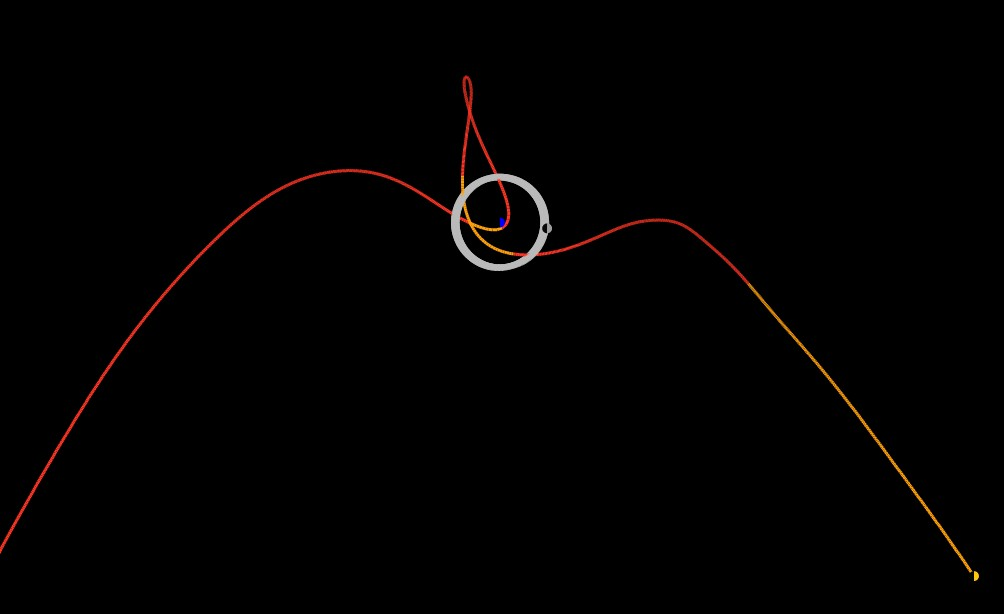
\includegraphics[width=\textwidth]{\PathToMedia/trajectories_2020SO.jpg}\\
		trajectories of objects in space \\
		\hyperref{https://en.wikipedia.org/wiki/2020_SO\#/media/File:2020SO_b.gif}{}{}{2020SO} 
	\end{minipage}
	\begin{minipage}[t]{0.25\textwidth}\centering
		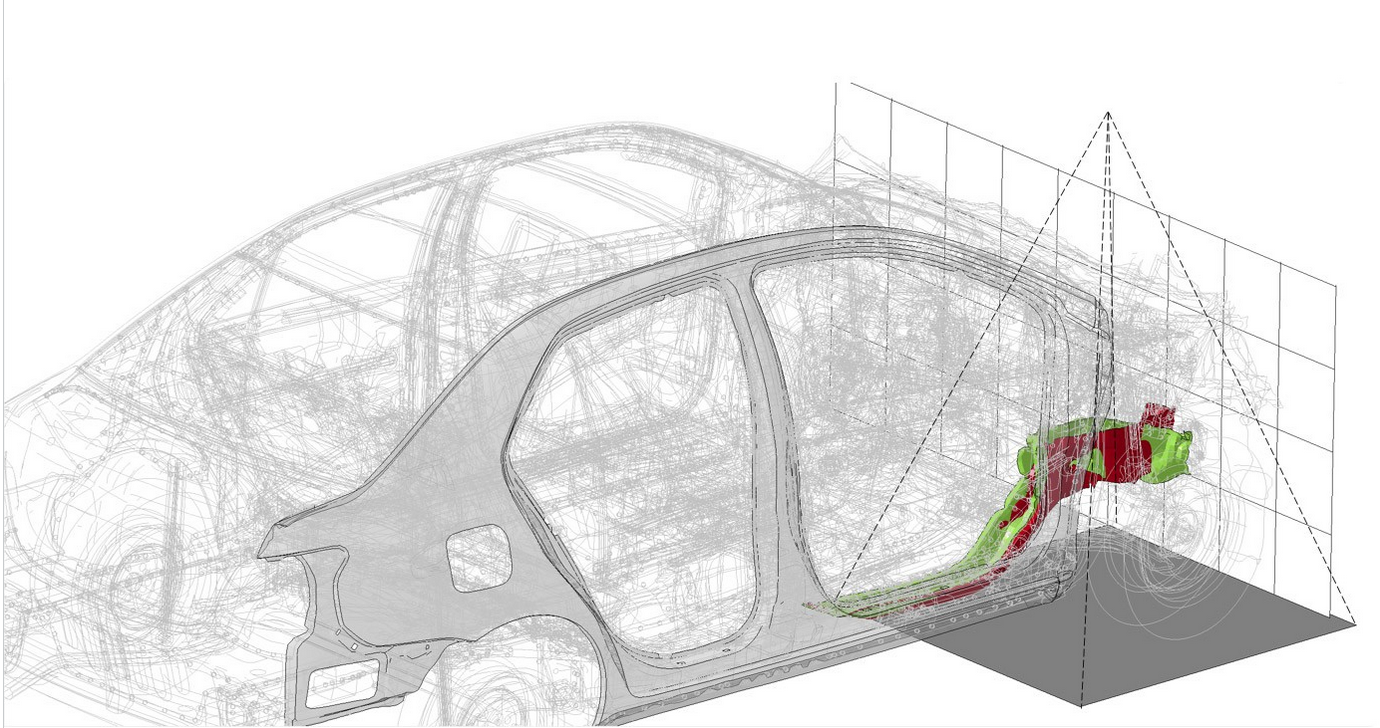
\includegraphics[width=\textwidth]{\PathToMedia/carcrash_sim.png}\\
		\hyperref{https://www.emi.fraunhofer.de/en/business-units/automotive/research/Roentgen-Crashtest.html}{}{}{car crash simulation} 
	\end{minipage}
	\begin{minipage}[t]{0.25\textwidth}\centering
		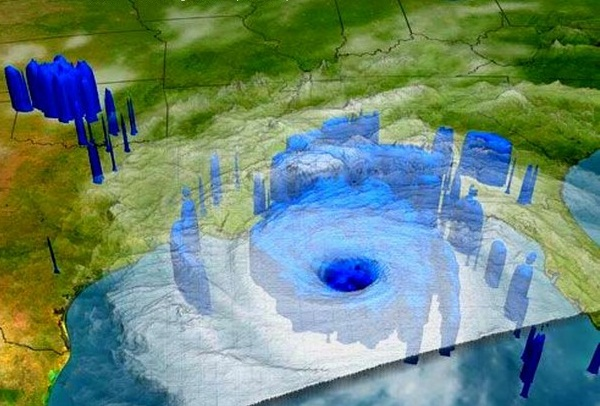
\includegraphics[width=\textwidth]{\PathToMedia/weather.jpg}\\
		\hyperref{https://en.wikipedia.org/wiki/Numerical_weather_prediction}{}{}{weather prediction} 
	\end{minipage}
	% CT SCAN
	\begin{minipage}[t]{0.25\textwidth} \centering
		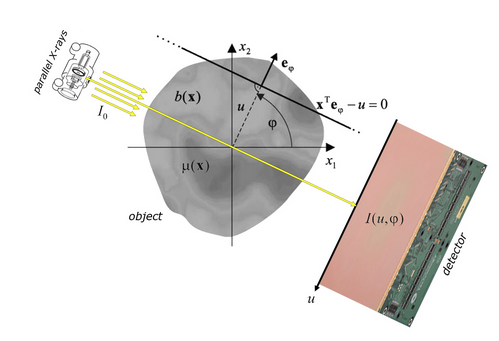
\includegraphics[width=\textwidth]{\PathToMedia/ct_scan.png}\\
		\hyperref{https://en.wikipedia.org/wiki/CT_scan}{}{}{CT Scan} 
	\end{minipage}
\end{frame}
%
%%%%%%%%%%%%%%%%%%%%%%%%%%%%%%%%%%%%%%%%%%%%%%%%%%%%%%%%%%%%%%%%%%%%%%%%%%%%%%%%%%
% CONTENT
%%%%%%%%%%%%%%%%%%%%%%%%%%%%%%%%%%%%%%%%%%%%%%%%%%%%%%%%%%%%%%%%%%%%%%%%%%%%%%%%%%
%\begin{frame}
%\textbf{\large \color{header} Content of the lecture}~\\\vspace{0.5cm}
%\begin{itemize}
%	\item \textbf{Basic Concepts of Linear Algebra}
%	\begin{itemize}
%		\item Sets, Mappings, Numbers, Sequences
%		\item Matrices, Norm, Determinant
%		\item QR-decomposition and the Gram-Schmidt algorithm
%	\end{itemize}
%	\item \textbf{Eigenvalues: Theory and Algorithms}
%	\begin{itemize}
%		\item The PageRank algorithm from Google
%		\item Eigendecomposition
%		\item Power method, reduction methods and the QR Algorithm
%	\end{itemize}
%	\item \textbf{Solving Linear Equations (of general size and dimensions)}
%	\begin{itemize}
%		\item Exact approaches and interpolation 
%		\begin{itemize}
%			\item Direct methods: Backward/Forward Substitution, Gaussian elimination, LU decomposition and QR decompositon
%			\item Iterative methods: Fixed Point Iterations (Richardson, Jacobi, Gauß-Seidel)
%		\end{itemize}
%		\item Approximate approaches and approximation 
%		\begin{itemize}
%			\item Linear Least Squares: Standard, Minimum-Norm Solution and Ridge Regression
%		\end{itemize}
%	\end{itemize}
%	\item \textbf{The Singular Value Decomposition: Theory and Applications}
%	\begin{itemize}
%		\item Theory
%		\item Applications: Data compression, pseudoinverse and least squares, Principal Component Analysis
%	\end{itemize}
%	\item \textbf{Vector Spaces}
%	\item \textbf{Krylov Subspace Methods} 
%	\item \textbf{Introductions to Nonlinear Aspects}
%	\begin{itemize}
%		\item Differentiation and Newton's method
%		\item Neural Networks
%	\end{itemize}
%\end{itemize}
%\end{frame}
%
\begin{frame}
	\textbf{\color{header} Preview}~\\\vspace{0.5cm}
	Let us assume we have $m$ data points
	$$(z_i, y_i),~~~i=1,\ldots,m,$$
	where
	\begin{itemize}
		\item $z_i$ are $n$-dimensional vectors of \textit{explanatory features} 
		\item $y_i$ are $k$-dimensional vectors representing the \textit{response/prediction/classification}
	\end{itemize}
	~\\
	$\rightarrow$ \textit{The term \textit{``vector''} already indicates that Linear Algebra comes naturally into the game.}
	~\\~\\~\\
	\textbf{Examples}\\
	\begin{itemize}
		\item You ask $m$ persons about 
		\begin{align*}
		z_i &= (\text{age}, \text{sex},\text{weight},\text{height},\text{years of experience}) &(n=5 ~ \text{dimensional vector})\\
		y_i &= \text{salary} &(k=1 ~ \text{dimensional vector})
		\end{align*}
		\item Consider $m$ years where
		\begin{align*}
		z_i &= \text{year} &(n=1 ~ \text{dimensional vector})\\
		y_i &= \text{global mean temperature} &(k=1 ~ \text{dimensional vector})
		\end{align*}	
		\item Consider $m$ images that you want to classify 
		\begin{align*}
		z_i &=(p_{lj})_{lj} & (\text{image stored as matrix/vector})\\
		y_i &= (\text{dog}, \text{cat}, \text{elephant}) &(k=3 ~ \text{dimensional vector})
		\end{align*}
	\end{itemize}
	
\end{frame}

\begin{frame}
	\textbf{\large \color{header} Dealing solely with the features $z$}~~\\~\\
	Applications of the \textbf{Singular Value Decomposition} are:\\
	% Consider just the $m$ $n$-dimensional feature vectors $z_i$:\\~\\
	~\\~\\
	\begin{minipage}[t]{0.48\textwidth}
		\textbf{Principal Component Analysis (PCA)}\\~\\
		{\raggedright
			$\rightarrow$ Aim: dimension reduction\\~\\}
		{\centering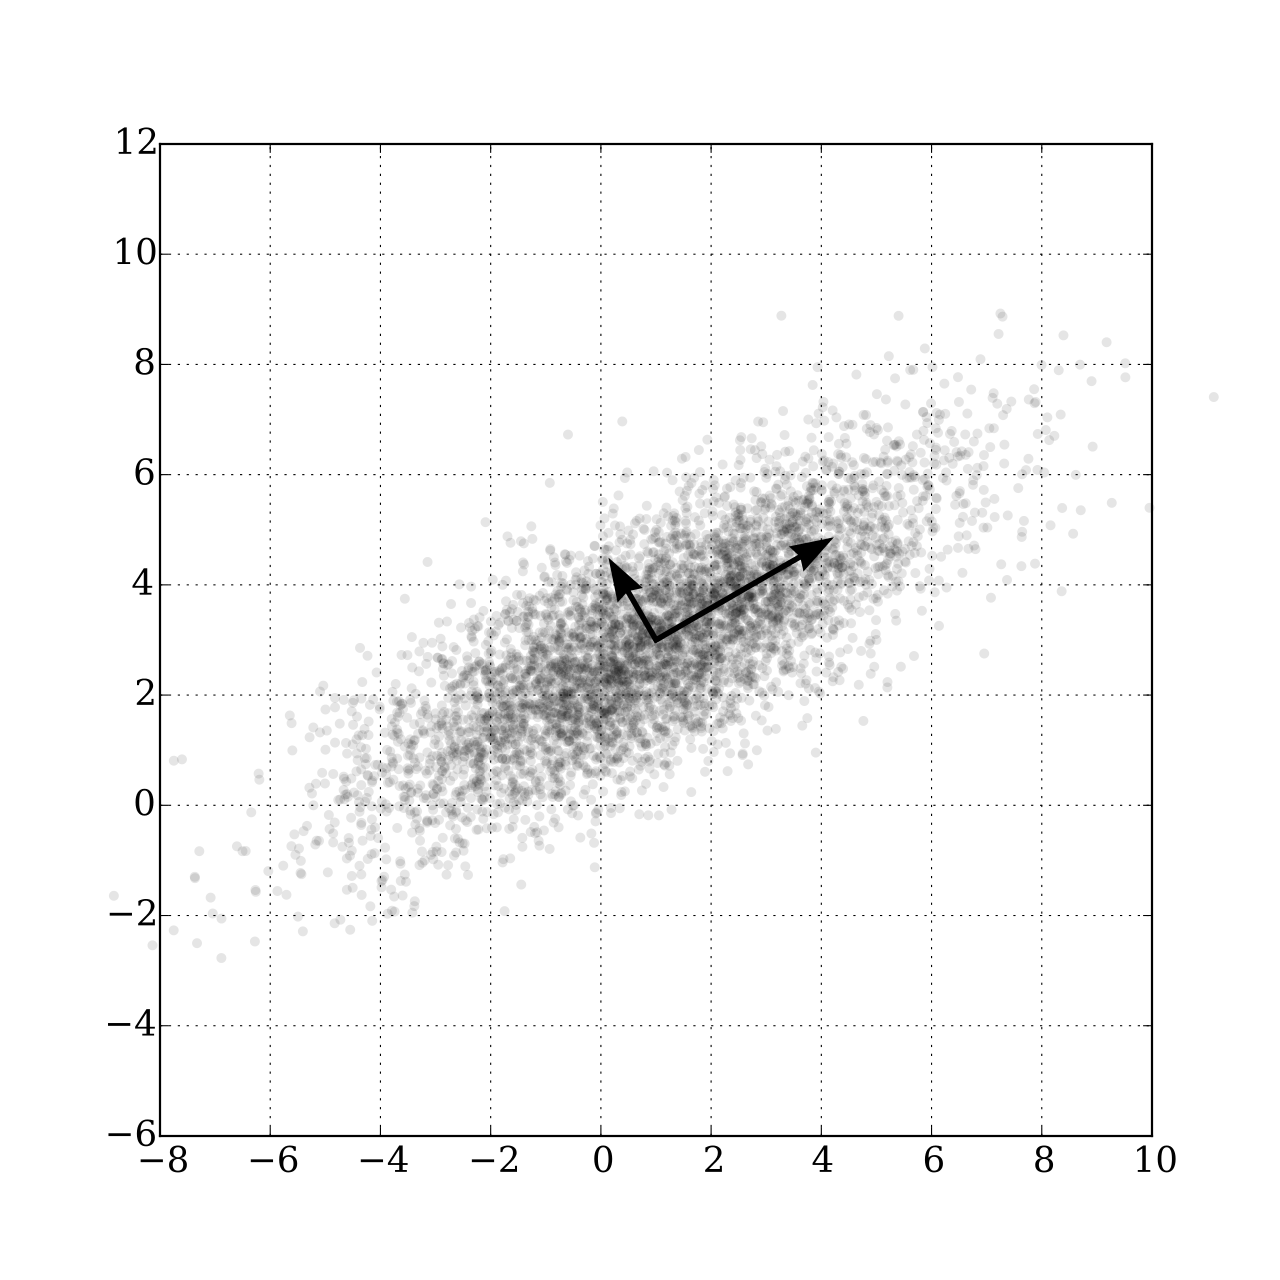
\includegraphics[width=0.77\textwidth]{\PathToMedia/PCA.png}}
	\end{minipage}
	~~~~~
	\begin{minipage}[t]{0.48\textwidth}
		\textbf{Data compression}\\~\\
		\raggedright
		$\rightarrow$ Aim: compression without dimension reduction\\~\\
		{ \hspace*{-0.6cm}\centering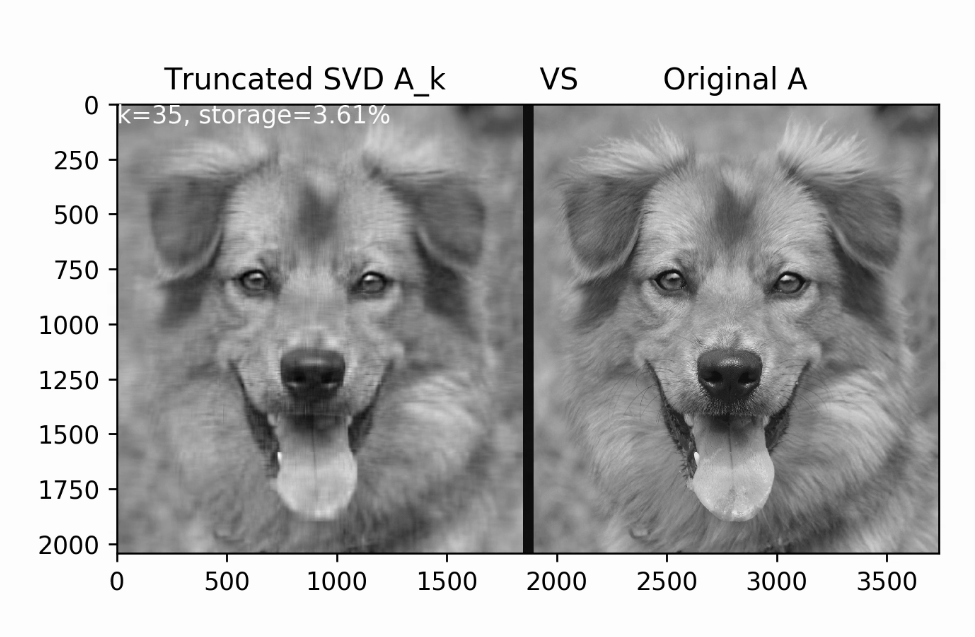
\includegraphics[width=1.1\textwidth]{\PathToMedia/SVD_dog.png}}
	\end{minipage}
\end{frame}
%
\begin{frame}
	\textbf{\large \color{header} Relating features $z$ to response $y$}~\\~\\
	One central goal in many scientific fields is to find a \textbf{model} $f_x$ depending on some parameters $x=(x_i)_i$, which ``best'' explains the relation between $z_i$ and $y_i$ in the sense that 
	$$f_x(z_i) \approx y_i,~~~\text{for all}~~i=1,\ldots,m$$
	\begin{itemize}
		\item  \textbf{The task:} Find those parameters $x$ for which the ``distance'' between our prediction  $f_x(z_i)$ and the measured response $y_i$ is ``as small as possible''\\
		\item \textbf{Our Toolbox:} Numerical Mathematics
		~\\
	\end{itemize}
	~\\~\\
	\textbf{Curve Fitting}\\
	 \centering	
		$$f_x(z) := x_0 + x_1z + x_2 z^2$$
		\\ \centering
		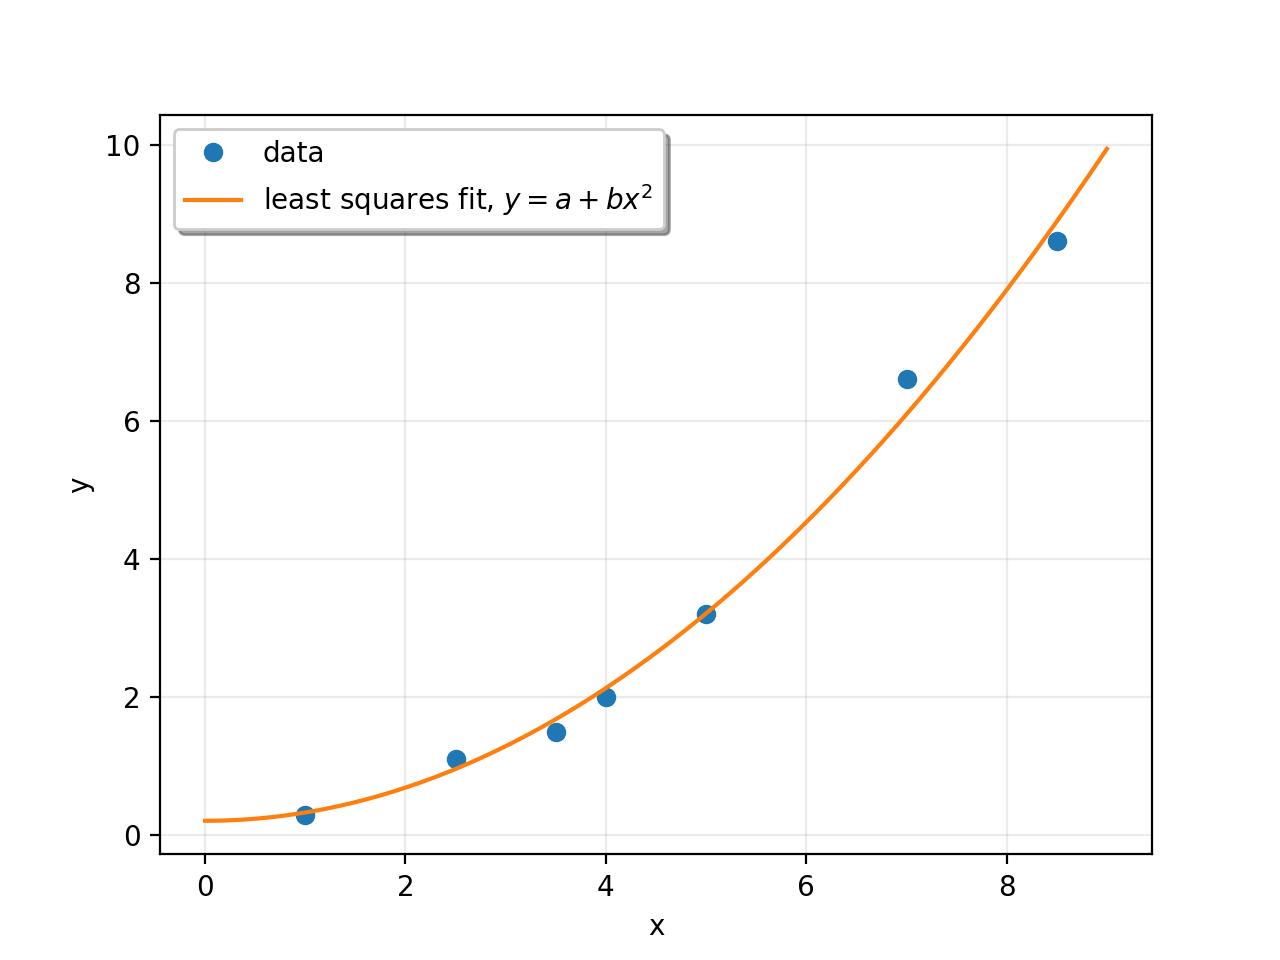
\includegraphics[width=0.37\textwidth]{\PathToMedia/4_least_squares.png}\\
\end{frame}

\begin{frame}
	~\\~\\
	\textbf{Simple image inpainting}\\
	$$\min_c \|Ac-b\|^2 + R(c)$$\\ \centering
	\begin{center}
		\hspace*{-0.3cm}	\includegraphics[width=1.00\textwidth]{\PathToMedia/Image_Inpainting.png}
	\end{center}
\end{frame}




%%%%%%%%%%%%%%%%%%%%%%%%%%%%%%%%%%%%%%%%%%%%%%%%%%%%%%%%%%%%%%%%%%%%%%%%%%%%%%%%%%
% BIBLIOGRAPHY
%%%%%%%%%%%%%%%%%%%%%%%%%%%%%%%%%%%%%%%%%%%%%%%%%%%%%%%%%%%%%%%%%%%%%%%%%%%%%%%%%%
%\begin{frame}
%\only<article>{\newpage}
%\textbf{\large \color{header} Literature}\\
%~\\
%\textbf{Main source} for this course:\\~\\ \vspace{1cm}
%	%LEFT
%\begin{minipage}[c]{0.4\textwidth}
%	\centering
%	\includegraphics[width=0.6\textwidth]{\PathToMedia/strang_learning.jpg}
%\end{minipage}
%%RIGHT
%\begin{minipage}[c]{0.6\textwidth}
%	\textit{\bf Linear Algebra and Learning from Data} \cite{StrangData} by Gilbert Strang\\
%\end{minipage}
%~\\~\\
%~\\ $\rightarrow$ contains basics of linear algebra, numerical linear algebra and finally an introduction to neural networks
%~\\ $\rightarrow$ we are currently trying to make it available as online ressource via the university library's platform \hyperref{https://tricat.uni-trier.de}{}{}{TRiCat}\footnote{https://tricat.uni-trier.de}
%\end{frame}
%%%
%\begin{frame}
%~\\~\\
% Besides this, inspiration is also taken from
% \begin{itemize}
% 	\item \cite{Deuflhard} (a classic textbook on numerical mathematics, in German)
% 	\item \cite{Rannacher} (lecture notes on numerical mathematics, also in German)
% \end{itemize}
%A classic textbook for numerical linear algebra is
%\begin{itemize}
%	\item  \cite{Golub} (worth being conducted, contains a rich list of other related literature)
%\end{itemize}
%~\\
%For those who prefer to learn a programming language via a proper textbook may want to have a look into 
%\begin{itemize}
%	\item \cite{Linge2020} (I recommend \hyperref{https://scipy-lectures.org/}{}{}{https://scipy-lectures.org/})
%\end{itemize}
%~\\\scriptsize
%\only<article>{\newpage}
%\pagestyle{plain}
%\bibliographystyle{abbrv}
%\bibliography{LocalFolder/literature_sparse}
%\nocite*{} 
%\end{frame}
%%%%%%%%%%%%%%%%%%%%%%%%%%%%%%%%%%
%%%%%%%%%%%%%%%%%%%%%%%%%%%%%%%%%%%%%%%%%%%%%%%%%%%%%%%%%%%%%%%%%%%%%%%%%%%%%%%%%%
% PYTHON
%%%%%%%%%%%%%%%%%%%%%%%%%%%%%%%%%%%%%%%%%%%%%%%%%%%%%%%%%%%%%%%%%%%%%%%%%%%%%%%%%%
%\begin{frame}
%\begin{columns}[t]
%	\begin{column}{0.7\textwidth}\vspace{-2.5cm}~\\
%	\textbf{\large \color{header} Python}\\~\\All programming related parts of this lecture will be presented and implemented using \textbf{Python 3}   
%	\end{column}
%	\begin{column}{0.3\textwidth}
%		\includegraphics[width=0.9\textwidth]{\PathToMedia/python.jpg}
%	\end{column}
%\end{columns}
%~\\
%\textbf{Why Python?}
%\begin{itemize}
%	\item universal, multi-purpose programming language
%	\item open source (!)
%	\item multi-platform (runs on all OS)
%	\item easy syntax, readable code (almost looks like pseudocode)
%\end{itemize}
%~\\
%\textbf{Some Background}
%\begin{itemize}
%	\item developed in 1990 by Guido van Rossum (Netherlands) -- name is homage to Monty Python
%\item interpreter programming language ($\neq$ compiled language such as C or Fortran)
%	\item used by: Google Mail, Google Maps, YouTube, Dropbox, ...
%	\item for scientific computing we use from the Scipy Stack: \textbf{SciPy} (2001), \textbf{NumPy} (1995,2006), \textbf{matplotlib} (2003)
%\end{itemize}
%\end{frame}
%%
%\begin{frame}
%~\\
%\textbf{Programming}
%\begin{itemize}
%	\item Basically every text editor can be used (nano, vi, geany, gedit,...)
%	\item For software development it is often more convient to use an \textbf{integrated development environment (IDE)} such as\\\vspace{0.1cm}~~~~~~~~~~~~~~~~~~
%	%LEFT
%	\begin{minipage}[c]{0.1\textwidth}
%		\centering\textbf{Spyder 3}\\
%		\includegraphics[width=0.6\textwidth]{\PathToMedia/spyder.png}
%	\end{minipage}
%	%RIGHT
%	\begin{minipage}[c]{0.1\textwidth}
%		\centering		\textbf{PyCharm}\\
%		\includegraphics[width=0.6\textwidth]{\PathToMedia/pycharm.png}
%	\end{minipage}
%\end{itemize}
%
%\begin{center}
%	\includegraphics[width=0.5\textwidth]{\PathToMedia/pycharm_screen.png}
%\end{center}
%\end{frame}
%%
%\begin{frame}
%~\\
%In this lecture we use: \textbf{\large \color{header} Jupyter Notebook}
%\begin{center}
%	\includegraphics[width=0.25\textwidth]{\PathToMedia/jupyter.png}
%\end{center}
%\begin{itemize}
%	\item open source, \textbf{web based} interactive environment\\
%	$\rightarrow$ thus multi-platform;\\
%	\item developed by \textbf{Project Juypter} (NPO)
%	\item name refers to \textbf{Ju}lia, \textbf{Pyt}hon, \textbf{R}
%	\item You can include: markdown, html, \LaTeX,...
%	\item and therefore also: images, pdfs, mathematical formulas,...
%	\item files can be exported as: html, slideshows, Latex .tex, PDF .pdf, ...
%\end{itemize}
%\end{frame}
%%
%\begin{frame}
%\textbf{\color{header}Advantages}\\\vspace{-0.5cm}
%\begin{center}
%	\includegraphics[width=0.6\textwidth]{\PathToMedia/Screen_ipynb.png}
%\end{center}
%\begin{itemize}
%	\item the whole process can be documented:
%	\begin{center}
%		Coding $\rightarrow$ Documentation $\rightarrow$ Run $\rightarrow$ Communication and Presentation
%	\end{center}
%	\item in fact, a jupyter notebook contains all the input \textbf{and} output of an interactive session plus additional text\\
%	$\rightarrow$ complete record!	
%\end{itemize}
%\end{frame}
%%
%\begin{frame}
%	\textbf{\large \color{header} Getting Started}\\\vspace{0.5cm}
%	\textbf{Installation}
%	\begin{center}
%		 \includegraphics[width=0.25\textwidth]{\PathToMedia/anaconda.png}
%	\end{center}
%	\begin{itemize}
%		\item We recommend to download the distribution \textbf{Anaconda} (\hyperref{https://www.anaconda.com/distribution/}{}{}{https://www.anaconda.com/distribution/}) \\
%		 $\rightarrow$ available for Linux, Windows, and Mac OS X ~\\ 
%		\item Comes along with:
%		\begin{itemize}
%			\item graphical user interface (\textit{Anaconda Navigator})
%			\item Spyder, Jupyter Notebook, RStudio (IDE for R)
%			\item installs all important packages (NumPy, SciPy, matplotlib, TensorFlow, scikit-learn,$\ldots$)
%			\item  package manager (\textit{Conda}) (standard is \textit{pip})
%		\end{itemize}
%	\end{itemize}
%~\\~\\
%\textbf{Tutorials}
%\begin{itemize}
%	\item Quickstart to Jupyter Notebook:
%	\begin{center}
%		\hyperref{https://scipy-lectures.org/}{}{}{https://scipy-lectures.org/}
%	\end{center}
%	\item Scientific computing with Python:
%	\begin{center}
%		\hyperref{https://jupyter.readthedocs.io/en/latest/content-quickstart.html}{}{}{https://jupyter.readthedocs.io/en/latest/content-quickstart.html}
%	\end{center}
%\end{itemize}	
%\end{frame}
%%
%\begin{frame}
%\textbf{\large \color{header} Summary}\\\vspace{0.5cm}
%\begin{itemize}
%	\item Check out the website\\
%	\begin{center}
%		 \slides 
%	\end{center} 
%	~\\
%	\item carefully read the information sheet
%	\begin{center}
%	\hyperref{https://www.math.uni-trier.de/~vollmann/elomath/organization.pdf}{}{}{	https://www.math.uni-trier.de/$\sim$vollmann/elomath/organization.pdf}
%	\end{center}
%	~\\
%	\item install anaconda on your machine and check out jupyter notebook
%	\begin{center}
%		\hyperref{https://www.anaconda.com/distribution/}{}{}{https://www.anaconda.com/distribution/}
%	\end{center}
%	~\\
%	\item getting started with Python and the Scipy Stack
%	\begin{center}
%		\hyperref{https://scipy-lectures.org/}{}{}{https://scipy-lectures.org/}
%	\end{center}
%	~\\
%	\item check out the course repository on olat and upload a ``hello world'' juypter notebook into the homework folder ``Test'' with the correct formatting for homework submissions 
%		\begin{center}
%		\hyperref{https://olat.vcrp.de/url/RepositoryEntry/2782398306/CourseNode/102353864883827}{}{}{https://olat.vcrp.de/url/RepositoryEntry/2782398306/CourseNode/102353864883827}
%	\end{center}
%	~\\  
%	\item prepare the first exercise sheet for submission next week and upload into homework folder ``1'' on olat
%		\begin{center}
%		\hyperref{https://www.math.uni-trier.de/~vollmann/elomath/sheets/1_sheet.pdf}{}{}{	https://www.math.uni-trier.de/$\sim$vollmann/elomath/build/1\_sheet.pdf}
%	\end{center}
%\end{itemize}
%\end{frame}




%%%%%%%%%%%%%%%%%%%%%%%%%%%%%%%%%%%%%%%%%%%%%%%%%%%%%%%%%%%%%%%%%%%%%%%%%%%%%%%%%%%
%% ORGANIZATION
%%%%%%%%%%%%%%%%%%%%%%%%%%%%%%%%%%%%%%%%%%%%%%%%%%%%%%%%%%%%%%%%%%%%%%%%%%%%%%%%%%%
%%\only<presentation>{
%%
%\begin{frame}
%\Section{Introduction}
%\Vspace{0.3cm}
%Always start here:
%\begin{center}
%\classMaterial
%\end{center}
%%
%\Vspace{0.5cm}
%You can log in using the following credentials:
%%
%\begin{center}
%	\htaccess
%\end{center}
%%
%\Vspace{1.0cm}
%In particular you will find an \textbf{information sheet}
%\begin{center}
%	\infoSheet
%\end{center}
% which contains \textbf{all} organizational information for this course (if you miss something please contact me:\\ \href{mailto:vollmann@uni-trier.de}{vollmann@uni-trier.de}).
%\end{frame}
%
%
%
%
%
%%%%%%%%%%%%%%%%%%%%%%%%%%%%%%%%%%%%%%%%%%%%%%%%%%%%%%%%%%%%%%%%%%%%%%%%%%%%%%%%%%%
%% APPETIZER
%%%%%%%%%%%%%%%%%%%%%%%%%%%%%%%%%%%%%%%%%%%%%%%%%%%%%%%%%%%%%%%%%%%%%%%%%%%%%%%%%%%
%%
%\begin{frame}
%%\textbf{\color{header} From the Module Handbook:}\\~\\
%%\textit{``After completing the module, the students know the mathematical foundations in the areas of linear algebra and \textbf{numerical mathematics}. As part of the course, they acquire or deepen knowledge in the programming language \textbf{Python}.''}\\
%~\\
%\textbf{Numerical mathematics?}\\
%\textit{Field of mathematics that deals with the construction and analysis of algorithms to approximately (but accurately) compute solutions to (hard) continuous problems -- typically using computers.}
%\Vspace{2cm}
%\textbf{\color{header} Why is this important?}~\\
%\begin{itemize}
%	\item most (all?) \textbf{application}-oriented problems cannot be solved exactly $\rightarrow$ \textit{\textbf{hard}} problems \Vspace{0.3cm}
%\end{itemize}
%\begin{minipage}[t]{0.25\textwidth}\centering
%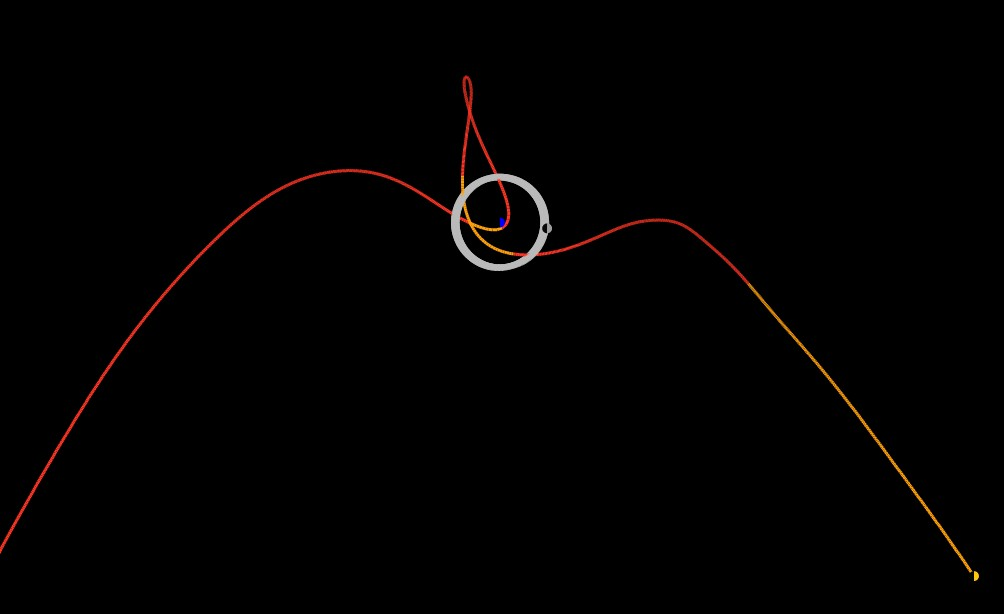
\includegraphics[width=\textwidth]{\PathToMedia/trajectories_2020SO.jpg}\\
%trajectories of objects in space \\
%	\hyperref{https://en.wikipedia.org/wiki/2020_SO\#/media/File:2020SO_b.gif}{}{}{2020SO} 
%\end{minipage}
%\begin{minipage}[t]{0.25\textwidth}\centering
%	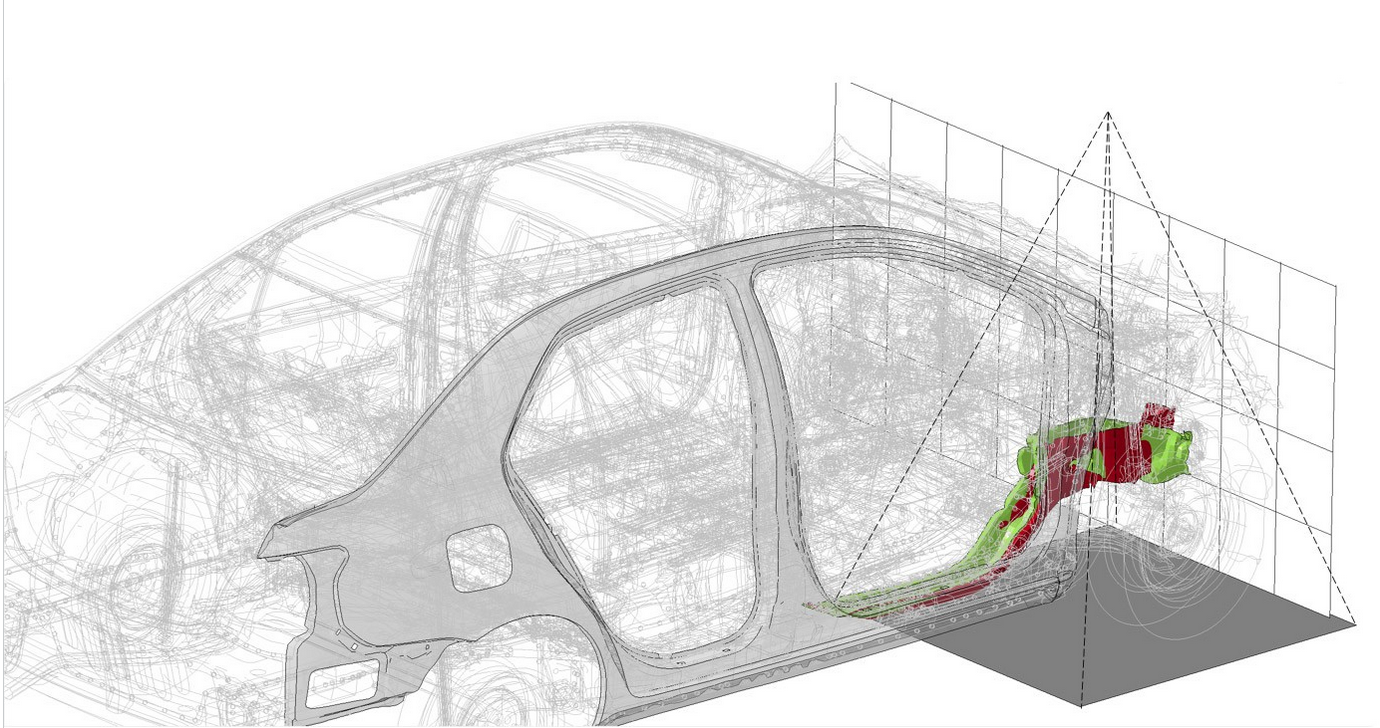
\includegraphics[width=\textwidth]{\PathToMedia/carcrash_sim.png}\\
%	\hyperref{https://www.emi.fraunhofer.de/en/business-units/automotive/research/Roentgen-Crashtest.html}{}{}{car crash simulation} 
%\end{minipage}
%\begin{minipage}[t]{0.25\textwidth}\centering
%	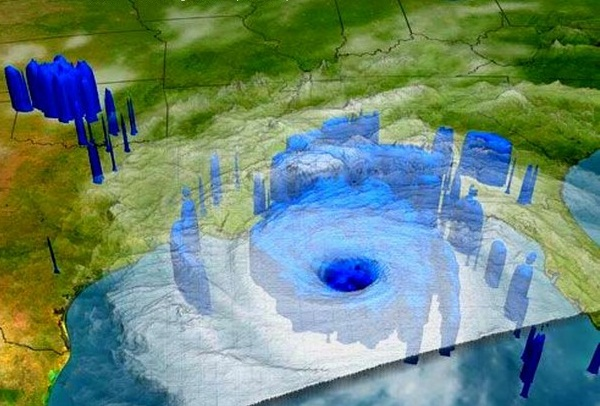
\includegraphics[width=\textwidth]{\PathToMedia/weather.jpg}\\
%	\hyperref{https://en.wikipedia.org/wiki/Numerical_weather_prediction}{}{}{weather prediction} 
%\end{minipage}
%% CT SCAN
%\begin{minipage}[t]{0.25\textwidth} \centering
%	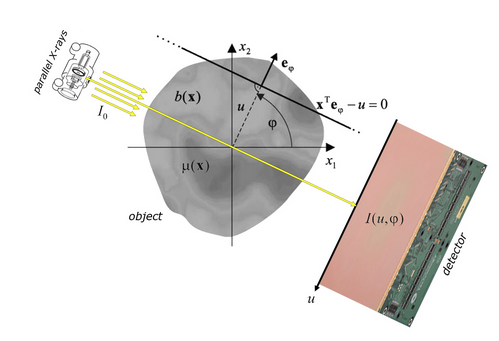
\includegraphics[width=\textwidth]{\PathToMedia/ct_scan.png}\\
%	\hyperref{https://en.wikipedia.org/wiki/CT_scan}{}{}{CT Scan} 
%\end{minipage}
%\end{frame}
%%
%\begin{frame}
%\textbf{\color{header} Relation to Data Science?}~\\
%\begin{itemize}
%\item \textbf{data}-driven models are more important than ever (due to the high amount of data available) \Vspace{0.2cm}
%\item data can be considered
%as a \textbf{mathematical object} (e.g., as a matrix/vector) \Vspace{0.2cm}
%\item with \textbf{numerical algorithms} we can manipulate data:\Vspace{0.2cm}
%\begin{itemize}\normalsize
%	\item solve systems involving the data (fitting data, prediction,...)
%	\Vspace{0.2cm}\item extract the most important features (singular values, PCA, data compression,...) 
%	\Vspace{0.2cm}\item calibrate models against data (machine learning, neural networks,...)
%\end{itemize}
%\end{itemize}
%
%~\\~\\
%\begin{minipage}[t]{0.25\textwidth}\centering
%	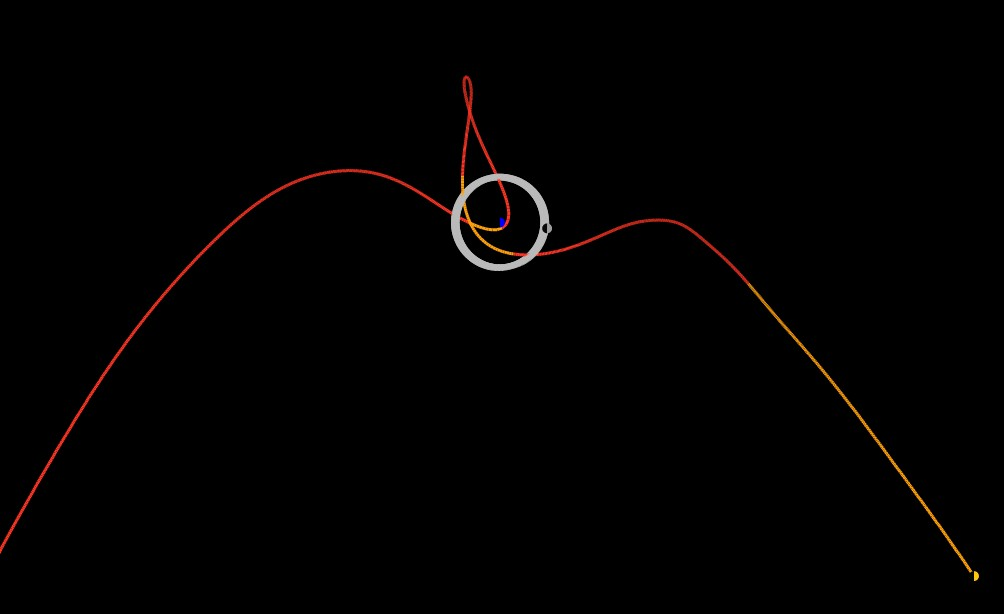
\includegraphics[width=\textwidth]{\PathToMedia/trajectories_2020SO.jpg}\\
%	trajectories of objects in space \\
%	\hyperref{https://en.wikipedia.org/wiki/2020_SO\#/media/File:2020SO_b.gif}{}{}{2020SO} 
%\end{minipage}
%\begin{minipage}[t]{0.25\textwidth}\centering
%	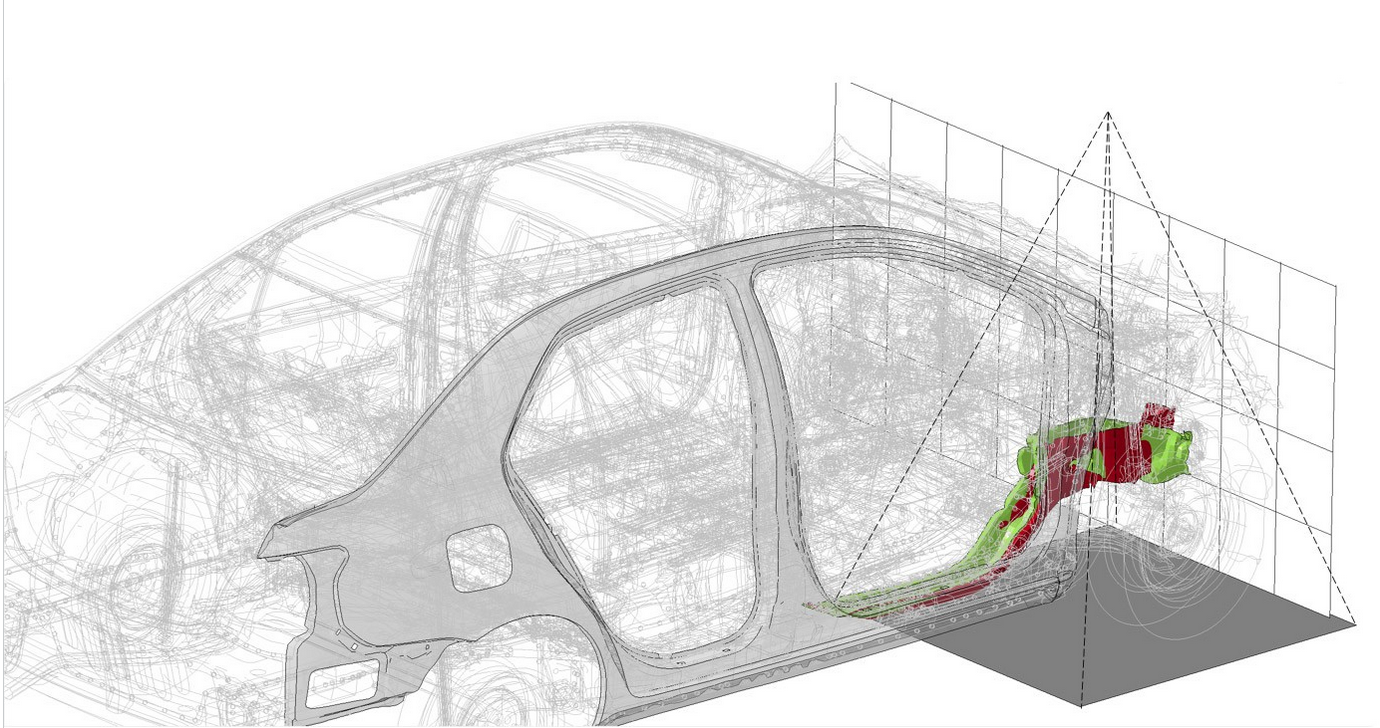
\includegraphics[width=\textwidth]{\PathToMedia/carcrash_sim.png}\\
%	\hyperref{https://www.emi.fraunhofer.de/en/business-units/automotive/research/Roentgen-Crashtest.html}{}{}{car crash simulation} 
%\end{minipage}
%\begin{minipage}[t]{0.25\textwidth}\centering
%	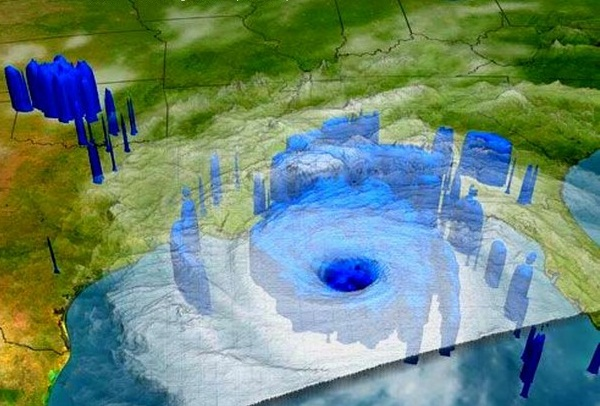
\includegraphics[width=\textwidth]{\PathToMedia/weather.jpg}\\
%	\hyperref{https://en.wikipedia.org/wiki/Numerical_weather_prediction}{}{}{weather prediction} 
%\end{minipage}
%% CT SCAN
%\begin{minipage}[t]{0.25\textwidth} \centering
%	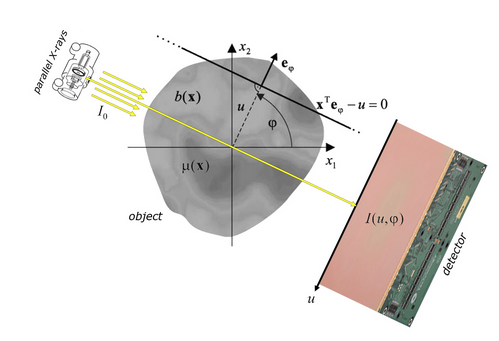
\includegraphics[width=\textwidth]{\PathToMedia/ct_scan.png}\\
%	\hyperref{https://en.wikipedia.org/wiki/CT_scan}{}{}{CT Scan} 
%\end{minipage}
%\end{frame}
%%
%%%%%%%%%%%%%%%%%%%%%%%%%%%%%%%%%%%%%%%%%%%%%%%%%%%%%%%%%%%%%%%%%%%%%%%%%%%%%%%%%%%
%% CONTENT
%%%%%%%%%%%%%%%%%%%%%%%%%%%%%%%%%%%%%%%%%%%%%%%%%%%%%%%%%%%%%%%%%%%%%%%%%%%
%
%%
%\begin{frame}
%\textbf{\color{header} Preview}~\\\Vspace{0.5cm}
%Let us assume we have $m$ data points
%$$(z_i, y_i),~~~i=1,\ldots,m,$$
%where
%\begin{itemize}
%	\item $z_i$ are $n$-dimensional vectors of \textit{explanatory features} 
%	\item $y_i$ are $k$-dimensional vectors representing the \textit{response/prediction/classification}
%\end{itemize}
%~\\
%$\rightarrow$ \textit{The term \textit{``vector''} already indicates that Linear Algebra comes naturally into the game.}
%~\\~\\~\\
%\textbf{Examples}\\
%\begin{itemize}
%	\item You ask $m$ persons about 
%	\begin{align*}
%			z_i &= (\text{age}, \text{sex},\text{weight},\text{height},\text{years of experience}) &(n=5 ~ \text{dimensional vector})\\
%	 y_i &= \text{salary} &(k=1 ~ \text{dimensional vector})
%	\end{align*}
%	\item Consider $m$ years where
%			\begin{align*}
%			z_i &= \text{year} &(n=1 ~ \text{dimensional vector})\\
%			y_i &= \text{global mean temperature} &(k=1 ~ \text{dimensional vector})
%			\end{align*}	
%	\item Consider $m$ images that you want to classify 
%			\begin{align*}
%			z_i &=(p_{lj})_{lj} & (\text{image stored as matrix/vector})\\
%			y_i &= (\text{dog}, \text{cat}, \text{elephant}) &(k=3 ~ \text{dimensional vector})
%			\end{align*}
%\end{itemize}
%
%\end{frame}
%
%\begin{frame}
%\textbf{\large \color{header} Dealing solely with the features $z$}~~\\~\\
% Applications of the \textbf{Singular Value Decomposition} are:\\
%% Consider just the $m$ $n$-dimensional feature vectors $z_i$:\\~\\
%~\\~\\
% \begin{minipage}[t]{0.48\textwidth}
% \textbf{\color{header}Principal Component Analysis (PCA)}\\~\\
% {\raggedright
%  $\rightarrow$ Aim: dimension reduction\\~\\}
%  {\centering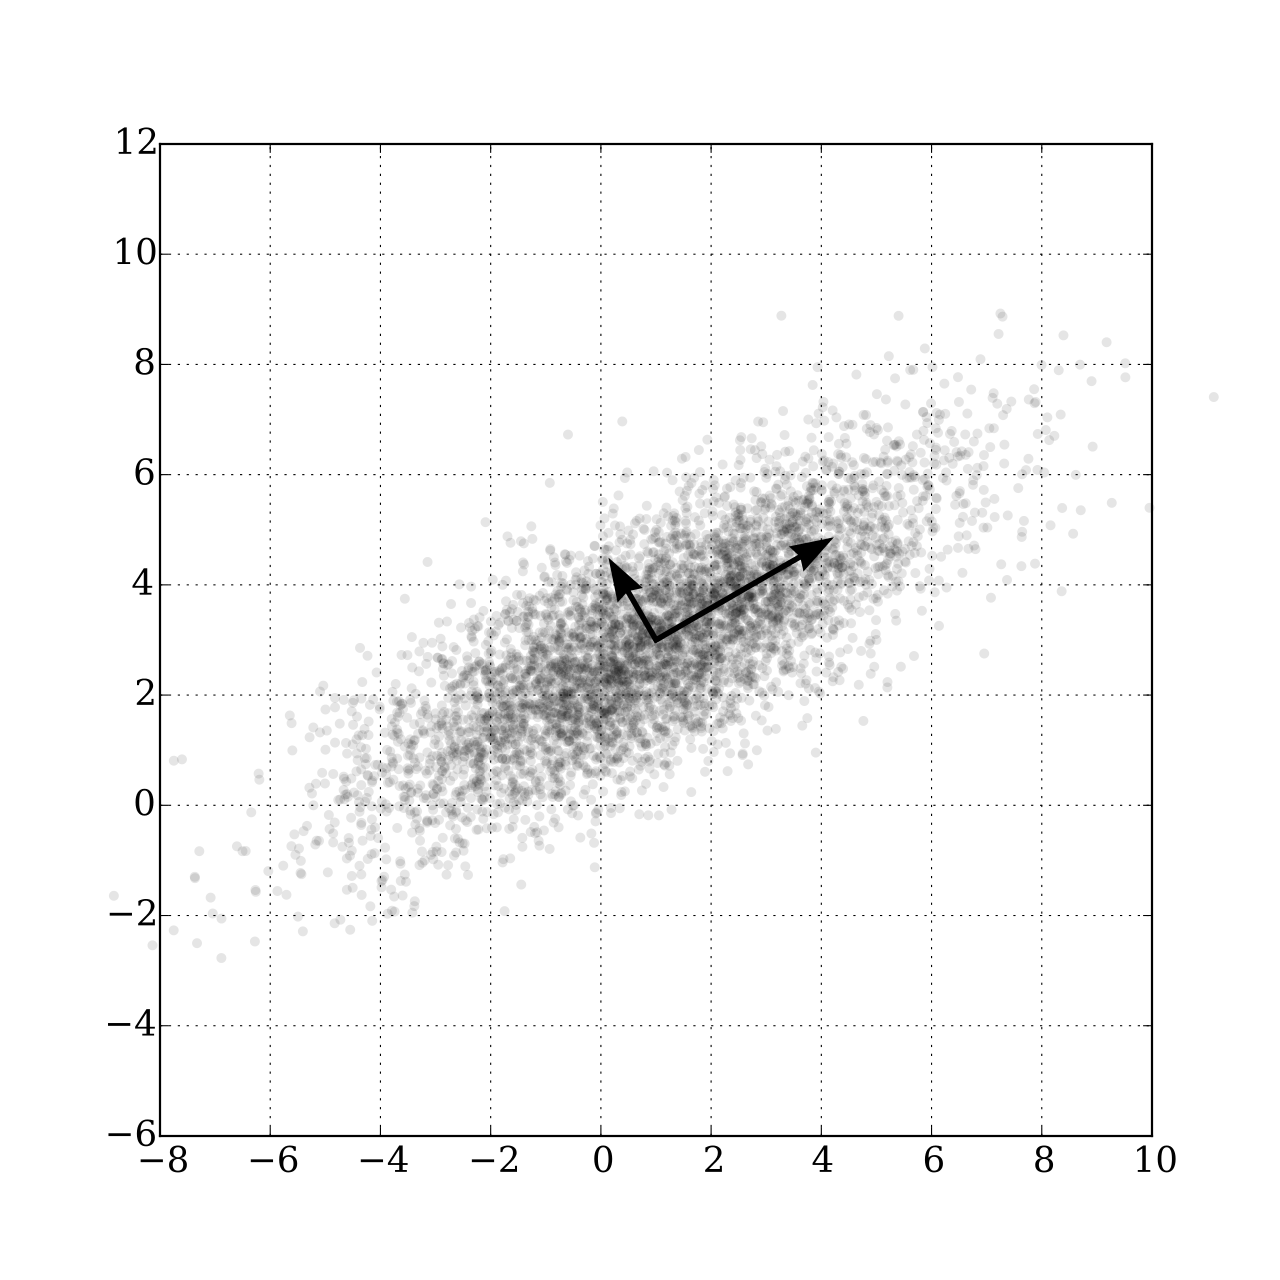
\includegraphics[width=0.7\textwidth]{\PathToMedia/PCA.png}}
% \end{minipage}
%~~~~~
% \begin{minipage}[t]{0.48\textwidth}
% \textbf{\color{header}Data compression}\\~\\
% \raggedright
% $\rightarrow$ Aim: compression without dimension reduction\\~\\
%{ \centering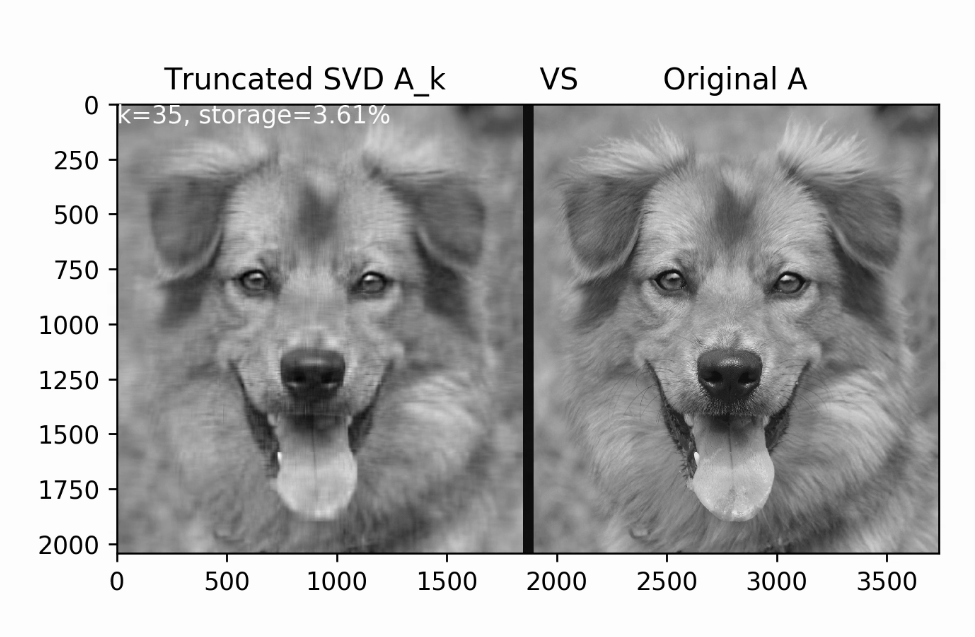
\includegraphics[width=0.99\textwidth]{\PathToMedia/SVD_dog.png}}
%\end{minipage}
%\end{frame}
%%
%\begin{frame}
%\textbf{\large \color{header} Relating features $z$ to response $y$}~\\~\\
%One central goal in data science is to find a \textbf{model} $f_c$ depending on some parameters $c$, which ``best'' explains the relation between $z_i$ and $y_i$ in the sense that 
%$$f_c(z_i) \approx y_i,~~~\text{for all}~~i=1,\ldots,n$$
%\begin{itemize}
%	\item  \textbf{The task:} Find those parameters $c$ for which the ``distance'' between our prediction  $f_c(z_i)$ and the measured response $y_i$ is ``as small as possible''\\
%	\item \textbf{Our Toolbox:} Numerical Mathematics
%	~\\
%\end{itemize}
%~\\
%\begin{minipage}[t]{0.4\textwidth}
%\textbf{\color{header}Solving linear systems:}\\ 
% $$f_c(z) := c_0 + c_1z + c_2 z^2$$\\ \centering
%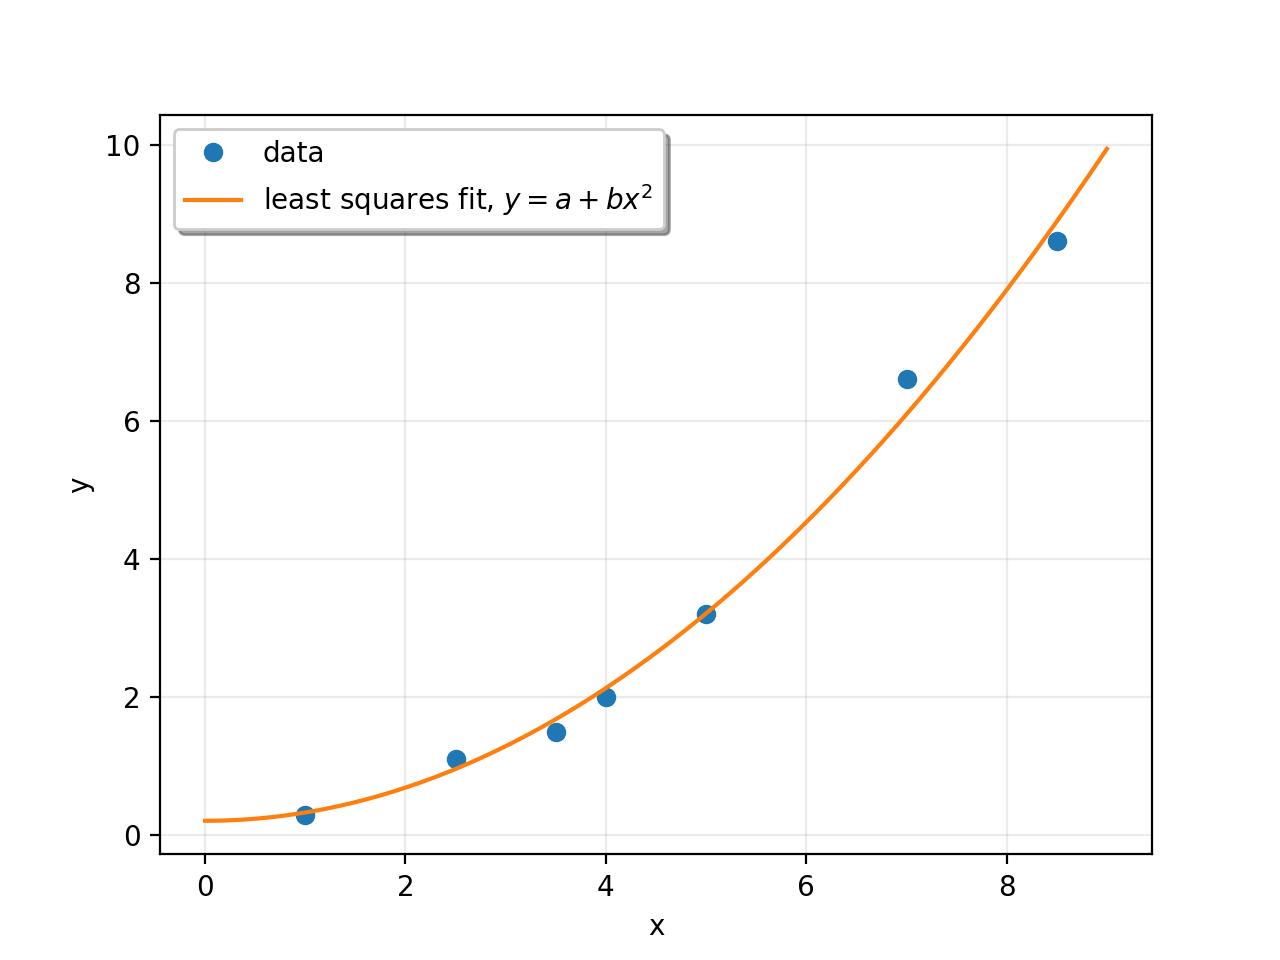
\includegraphics[width=0.8\textwidth]{\PathToMedia/4_least_squares.png}\\
%\end{minipage}
%%
%\begin{minipage}[t]{0.6\textwidth}
%\textbf{\color{header}Solving nonlinear systems:}\\
%Complicated ($\neq$ linear) relation between model and parameter\\
% $$f_c(z) := \textbf{Neural Network}_c(z)$$\\
%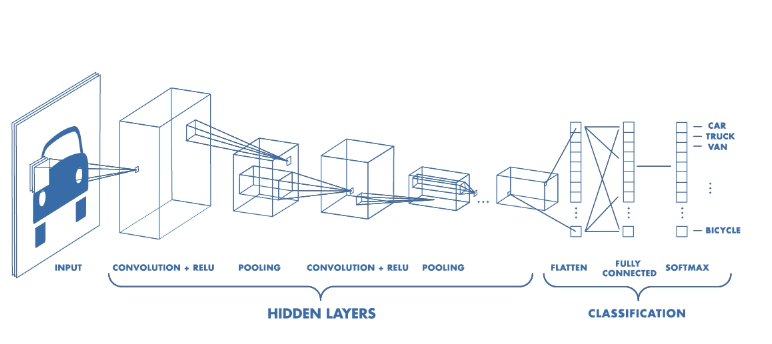
\includegraphics[width=0.59\textwidth]{\PathToMedia/CNN.png}
%\includegraphics[width=0.4\textwidth]{\PathToMedia/MNIST-DataSet.png}
%\end{minipage}
%\end{frame}
%
%
%%%%%%%%%%%%%%%%%%%%%%%%%%%%%%%%%%%
%%%%%%%%%%%%%%%%%%%%%%%%%%%%%%%%%%%%%%%%%%%%%%%%%%%%%%%%%%%%%%%%%%%%%%%%%%%%%%%%%%%
%% PYTHON
%%%%%%%%%%%%%%%%%%%%%%%%%%%%%%%%%%%%%%%%%%%%%%%%%%%%%%%%%%%%%%%%%%%%%%%%%%%%%%%%%%%
%\begin{frame}
%\begin{columns}[t]
%	\begin{column}{0.7\textwidth}\Vspace{-2.5cm}~\\
%	\textbf{\large \color{header} Python}\\~\\All programming related parts of this lecture will be presented and implemented using \textbf{Python 3}   
%	\end{column}
%	\begin{column}{0.3\textwidth}
%		\includegraphics[width=0.9\textwidth]{\PathToMedia/python.jpg}
%	\end{column}
%\end{columns}
%~\\
%\textbf{Why Python?}
%\begin{itemize}
%	\item universal, multi-purpose programming language
%	\item open source (!)
%	\item multi-platform (runs on all OS)
%	\item easy syntax, readable code (almost looks like pseudocode)
%\end{itemize}
%~\\
%\textbf{Some Background}
%\begin{itemize}
%	\item developed in 1990 by Guido van Rossum (Netherlands) -- name is homage to Monty Python
%\item interpreter programming language ($\neq$ compiled language such as C or Fortran)
%	\item used by: Google Mail, Google Maps, YouTube, Dropbox, ...
%	\item for scientific computing we use from the Scipy Stack: \textbf{SciPy} (2001), \textbf{NumPy} (1995,2006), \textbf{matplotlib} (2003)
%\end{itemize}
%\end{frame}
%%
%\begin{frame}
%~\\
%\textbf{Programming}
%\begin{itemize}
%	\item Basically every text editor can be used (nano, vi, geany, gedit, atom, emacs...)
%	\item For software development it is often more convient to use an \textbf{integrated development environment (IDE)} such as\\\Vspace{0.1cm}~~~~~~~~~~~~~~~~~~
%	%LEFT
%	\begin{minipage}[c]{0.1\textwidth}
%		\centering\textbf{Spyder 3}\\
%		\includegraphics[width=0.6\textwidth]{\PathToMedia/spyder.png}
%	\end{minipage}
%	%RIGHT
%	\begin{minipage}[c]{0.1\textwidth}
%		\centering		\textbf{PyCharm}\\
%		\includegraphics[width=0.6\textwidth]{\PathToMedia/pycharm.png}
%	\end{minipage}
%\end{itemize}
%
%\begin{center}
%	\includegraphics[width=0.5\textwidth]{\PathToMedia/pycharm_screen.png}
%\end{center}
%\end{frame}
%%
%\begin{frame}
%~\\
%In this lecture we will sometimes use: \textbf{\large \color{header} Jupyter Notebook}
%\begin{center}
%	\includegraphics[width=0.25\textwidth]{\PathToMedia/jupyter.png}
%\end{center}
%\begin{itemize}
%	\item open source, \textbf{web based} interactive environment\\
%	$\rightarrow$ thus multi-platform;\\
%	\item developed by \textbf{Project Juypter} (NPO)
%	\item name refers to \textbf{Ju}lia, \textbf{Pyt}hon, \textbf{R}
%	\item You can include: markdown, html, \LaTeX,...
%	\item and therefore also: images, pdfs, mathematical formulas,...
%	\item files can be exported as: html, slideshows, Latex .tex, PDF .pdf, ...
%\end{itemize}
%\end{frame}
%%
%\begin{frame}
%\textbf{\color{header}Advantages}\\\Vspace{-0.5cm}
%\begin{center}
%	\includegraphics[width=0.6\textwidth]{\PathToMedia/Screen_ipynb.png}
%\end{center}
%\begin{itemize}
%	\item the whole process can be documented:
%	\begin{center}
%		Coding $\rightarrow$ Documentation $\rightarrow$ Run $\rightarrow$ Communication and Presentation
%	\end{center}
%	\item in fact, a jupyter notebook contains all the input \textbf{and} output of an interactive session plus additional text\\
%	$\rightarrow$ complete record!	
%\end{itemize}
%\end{frame}
%%
%\begin{frame}
%	\textbf{\large \color{header} Getting Started}\\\Vspace{0.5cm}
%	\textbf{Installation}
%	\begin{center}
%		 \includegraphics[width=0.25\textwidth]{\PathToMedia/anaconda.png}
%	\end{center}
%	\begin{itemize}
%		\item I recommend to download the distribution \textbf{Anaconda} (\hyperref{https://www.anaconda.com/distribution/}{}{}{https://www.anaconda.com/distribution/}) \\
%		 $\rightarrow$ available for Linux, Windows, and Mac OS X ~\\ 
%		\item Comes along with:
%		\begin{itemize}
%			\item graphical user interface (\textit{Anaconda Navigator})
%			\item Spyder, Jupyter Notebook, RStudio (IDE for R)
%			\item installs all important packages (NumPy, SciPy, matplotlib, TensorFlow, scikit-learn,$\ldots$)
%			\item  package manager (\textit{Conda}) (standard is \textit{pip})
%		\end{itemize}
%	\end{itemize}
%~\\~\\
%\textbf{Tutorials}
%\begin{itemize}
%	\item Quickstart to Jupyter Notebook:
%	\begin{center}
%			\hyperref{https://jupyter.readthedocs.io/en/latest/content-quickstart.html}{}{}{https://jupyter.readthedocs.io/en/latest/content-quickstart.html}
%	\end{center}
%	\item Scientific computing with Python:
%	\begin{center}
%				\hyperref{https://scipy-lectures.org/}{}{}{https://scipy-lectures.org/}
%	\end{center}
%\end{itemize}	
%\end{frame}
%%
%\begin{frame}
%\textbf{\large \color{header} Summary}\\\Vspace{0.5cm}
%\begin{itemize}
%	\item Check out the website\\
%	\begin{center}
%		 \slides 
%	\end{center} 
%	~\\
%	\item if has not happened so far, carefully read the information sheet
%	\begin{center}
%	\infoSheet
%	\end{center}
%	~\\
%	\item install anaconda on your machine and check out jupyter notebook and Spyder
%	\begin{center}
%		\hyperref{https://www.anaconda.com/distribution/}{}{}{https://www.anaconda.com/distribution/}
%	\end{center}
%	~\\
%	\item alternatively: install the IDE \pycharm
%\begin{itemize}
%	\item set up jetbrains account via university account:\\
%\url{https://www.jetbrains.com/shop/eform/students2}
%	\item Download Professional Edition\\  \url{https://www.jetbrains.com/help/pycharm/installation-guide.html}
%\end{itemize}
%~\\
%	\item getting started with Python and the Scipy Stack
%	\begin{center}
%		\hyperref{https://scipy-lectures.org/}{}{}{https://scipy-lectures.org/}
%	\end{center}
%%	~\\
%%	\item check out the course repository on olat and upload a ``hello world'' juypter notebook into the homework folder ``Test'' with the correct formatting for homework submissions 
%%		\begin{center}
%%		\hyperref{https://olat.vcrp.de/url/RepositoryEntry/2782398306/CourseNode/102353864883827}{}{}{https://olat.vcrp.de/url/RepositoryEntry/2782398306/CourseNode/102353864883827}
%%	\end{center}
%%	~\\  
%	\item prepare the first exercise sheet 
%%	for submission next week and upload into homework folder ``1'' on olat
%%		\begin{center}
%%		\hyperref{https://www.math.uni-trier.de/~vollmann/elomath/sheets/1_sheet.pdf}{}{}{	https://www.math.uni-trier.de/$\sim$vollmann/elomath/build/1\_sheet.pdf}
%%	\end{center}
%\end{itemize}
%\end{frame}